\documentclass[10pt]{article}

\usepackage[margin=1in]{geometry}
\usepackage{booktabs}
\usepackage{graphicx}
\usepackage{hyperref}
\usepackage{amsmath}
\usepackage{caption}
\usepackage{subcaption}
\usepackage{enumitem}
\usepackage{xcolor}

\hypersetup{colorlinks=true, linkcolor=blue, citecolor=blue, urlcolor=blue}
\setlength{\parindent}{0pt}
\setlength{\parskip}{6pt}

\title{Computer Vision HW3: 2DGS/AIGC Scene Fusion and ACT Cross-Environment Generalization}
\author{
Student Name 1, Student ID 1 \\
Student Name 2, Student ID 2 \\
\textit{Work split: fill in concrete contributions before submission}
}
\date{June 2026}

\begin{document}
\maketitle

\textbf{GitHub:} \url{https://github.com/your-account/cv-hw3} \\
\textbf{Model weights:} \url{https://your-cloud-link.example.com}

\section{Task 1: Multi-Source 3D Asset Generation and Scene Fusion}

\subsection{Goal and Data}
The required final run reconstructs one real object from phone-captured multi-view imagery, generates one text-conditioned 3D object with SDS, generates one single-image-conditioned 3D object with Magic123, and inserts all three assets into a 2DGS-reconstructed Mip-NeRF 360 scene~\cite{barron2022mipnerf360,huang2024twodgs,qian2024magic123}. The repository contains the full scripts for this pipeline. Because the phone-captured object A video/photos and object C foreground image were not present in the workspace, the checked run below uses synthetic proxy meshes to verify the representation-unification, statistics, and Blender fusion/rendering stages. In addition, a synthetic NeRF-style object was trained with 2DGS for 200 iterations and exported through the official mesh extraction path, producing a 2666-vertex, 4968-face smoke-test mesh. A public NerfBaselines Mip-NeRF 360 sparse garden-n24 thumbnail dataset~\cite{nerfbaselines2024} was also converted to 2DGS format, trained for 300 iterations, and exported as an unbounded background mesh with 1,768,391 vertices and 3,563,531 faces. These proxy and smoke-test files must be replaced by real phone-object and full-resolution Mip-NeRF 360 outputs before final submission.

\subsection{Methods}
\textbf{Object A.} We extract frames from a phone video or multi-view image set, estimate camera poses with COLMAP, and optimize a 2D Gaussian Splatting model.

\textbf{Object B.} We use threestudio DreamFusion with Stable Diffusion guidance and SDS loss. The optimized implicit representation is exported as a textured mesh.

\textbf{Object C.} We remove the background from a single object photo, preprocess depth/foreground for Magic123, and run coarse NeRF and fine DMTet stages.

\textbf{Background.} We reconstruct the selected Mip-NeRF 360 scene with 2DGS and extract an unbounded TSDF mesh. The checked public-data smoke run uses low-resolution NerfBaselines garden-n24 thumbnails to validate conversion, 2DGS training, and unbounded mesh extraction without requiring the full 12.5GB archive.

\subsection{Representation Unification}
2DGS assets and the background are exported with the official 2DGS rendering/mesh extraction pipeline. AIGC assets are exported as OBJ/MTL meshes. We use textured meshes as the common representation and compose them in Blender. This avoids mixing surfel rasterization with implicit fields at render time and makes scale, rotation, and placement explicit.

\subsection{Results}
\begin{figure}[h]
  \centering
  \IfFileExists{figures/task1_fusion_preview.png}{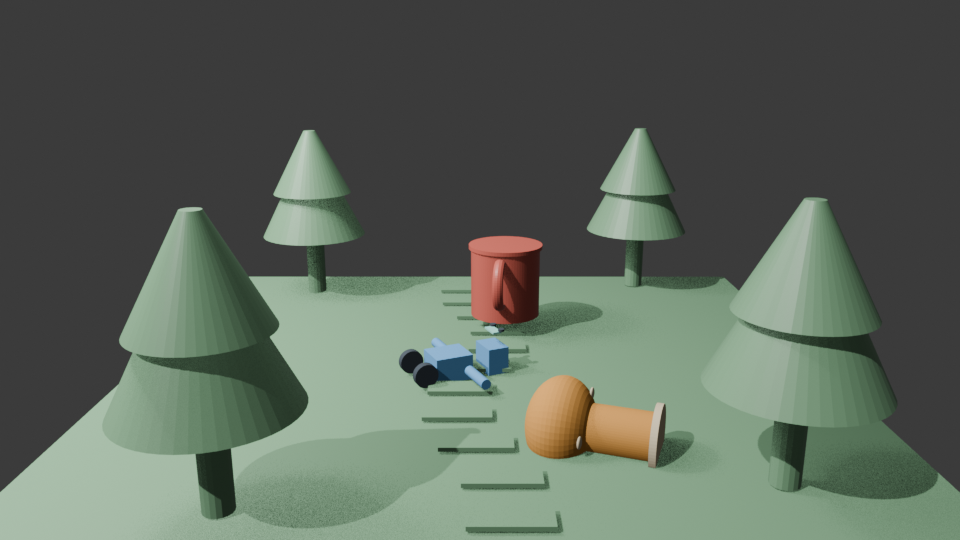
\includegraphics[width=0.82\linewidth]{figures/task1_fusion_preview.png}}{\fbox{\parbox{0.82\linewidth}{Task 1 fusion preview placeholder}}}
  \caption{Rendered demo fusion preview. The generated video is \texttt{results/task1/fusion\_demo/fusion\_walkthrough.mp4}, 960$\times$540, 72 frames at 24 fps.}
\end{figure}

\begin{figure}[h]
  \centering
  \IfFileExists{figures/task1_asset_mesh_stats.pdf}{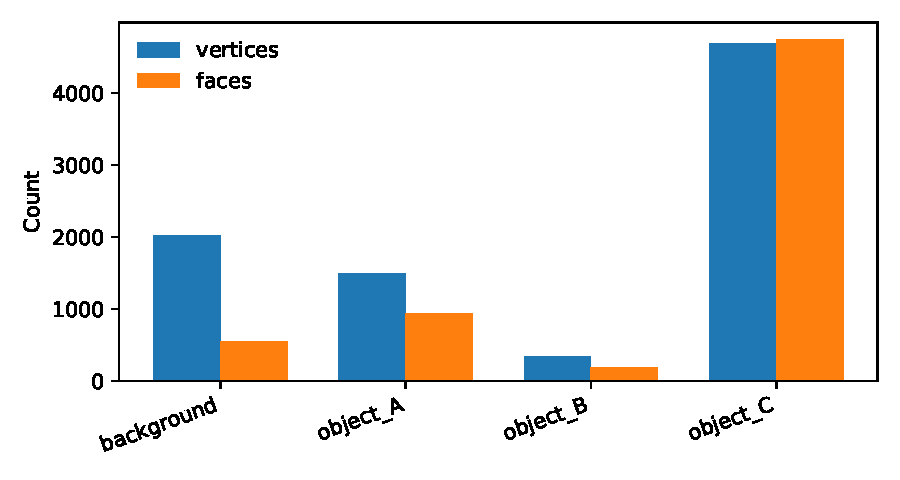
\includegraphics[width=0.75\linewidth]{figures/task1_asset_mesh_stats.pdf}}{\fbox{\parbox{0.75\linewidth}{Task 1 asset statistics figure placeholder}}}
  \caption{Mesh complexity of the current demo assets.}
\end{figure}

\begin{table}[h]
\centering
\caption{Current asset statistics and expected real-run behavior.}
\begin{tabular}{p{0.28\linewidth}rrp{0.36\linewidth}}
\toprule
Asset & Vertices & Faces & Notes \\
\midrule
Background proxy & 2016 & 552 & replace with 2DGS Mip-NeRF 360 mesh \\
Background sparse 2DGS smoke & 1768391 & 3563531 & NerfBaselines garden-n24 thumbnails, 300-step chain test \\
Object A proxy & 1489 & 932 & replace with phone multi-view 2DGS object \\
Object A 2DGS smoke & 2666 & 4968 & synthetic NeRF views, 200-iteration chain test \\
Object B proxy & 344 & 190 & replace with threestudio SDS export \\
Object C proxy & 4680 & 4740 & replace with Magic123 export \\
\bottomrule
\end{tabular}
\end{table}

\section{Task 2: ACT Cross-Environment Generalization on CALVIN}

\subsection{Setup}
We use CALVIN data released in HuggingFace LeRobot v2.1 format and convert local parquet subsets to LeRobot v3.0~\cite{mees2022calvin}. The B-only subset is inferred from the official CALVIN scene order within the ABCD dataset because the HF metadata does not expose an explicit environment label per episode. The checked run trains policies on 30 inferred-B episodes (1792 frames) and on a 7-episode ABC subset (386 frames), then evaluates both 100-step and 500-step checkpoints zero-shot on 20 D episodes (1267 frames). A later attempt to download a larger 40-episode ABC subset stalled after two episodes because of network throughput, so the ABC result is explicitly a small-data run.

\subsection{ACT Policy}
ACT predicts chunks of future actions using a Transformer policy~\cite{zhao2023act}. The chunking mechanism reduces compounding error by generating temporally coherent action sequences, but it can still be sensitive to visual distribution shift when the image encoder maps new scene appearances to out-of-training features.

\subsection{Hyperparameters}
\begin{table}[h]
\centering
\caption{ACT training hyperparameters.}
\begin{tabular}{lp{0.62\linewidth}}
\toprule
Item & Value \\
\midrule
Policy & LeRobot ACT \\
Network architecture & ResNet18 visual encoder + ACT Transformer, 52M parameters \\
Observations & robot state, top RGB image, wrist RGB image \\
Action chunk size & 100 \\
Batch size & 8 \\
Steps & 100 and 500 for checked runs; scripts default to 100000 \\
Optimizer & AdamW, learning rate $1\times10^{-5}$, weight decay $1\times10^{-4}$ \\
Loss & Action L1 + VAE KL auxiliary loss \\
Logging & Local LeRobot stdout logs captured under \texttt{results/task2/logs}; WandB disabled in the checked run \\
\bottomrule
\end{tabular}
\end{table}

\subsection{Training Curves and Zero-Shot Results}
\begin{figure}[h]
  \centering
  \IfFileExists{figures/task2_training_loss.pdf}{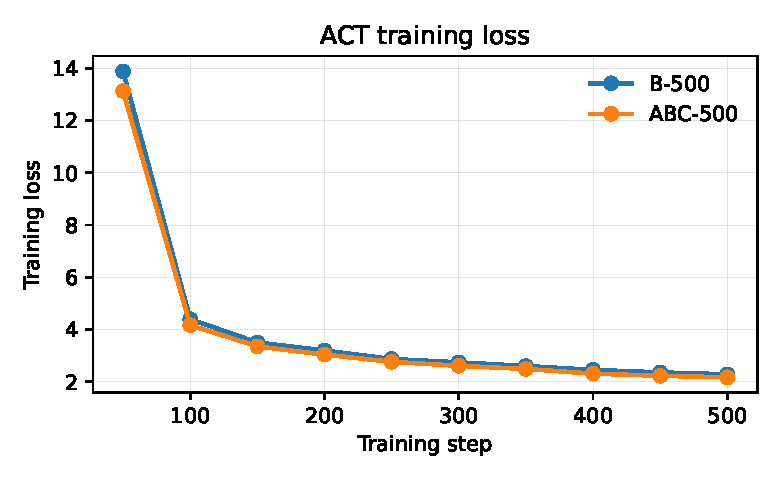
\includegraphics[width=0.62\linewidth]{figures/task2_training_loss.pdf}}{\fbox{\parbox{0.62\linewidth}{Task 2 training loss figure placeholder}}}
  \caption{ACT training loss from the checked 500-step B-only and ABC-small runs.}
\end{figure}

\begin{figure}[h]
  \centering
  \IfFileExists{figures/task2_action_l1.pdf}{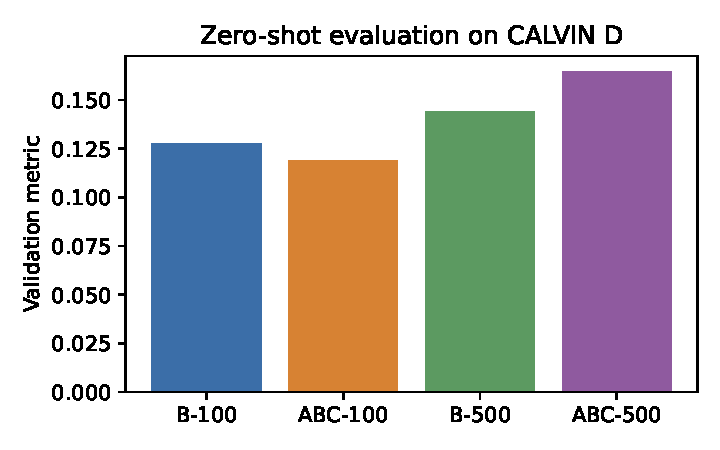
\includegraphics[width=0.6\linewidth]{figures/task2_action_l1.pdf}}{\fbox{\parbox{0.6\linewidth}{Task 2 Action L1 figure placeholder}}}
  \caption{Zero-shot validation metric on CALVIN environment D. Lower is better for Action L1.}
\end{figure}

\begin{table}[h]
\centering
\caption{Zero-shot evaluation on unseen environment D.}
\begin{tabular}{lrl}
\toprule
Policy & Action L1 $\downarrow$ & Notes \\
\midrule
ACT trained on inferred B & 0.1276 & 20 D batches, 100-step checkpoint \\
ACT trained on ABC-small & 0.1190 & 20 D batches, 100-step checkpoint \\
ACT trained on inferred B & 0.1442 & 20 D batches, 500-step checkpoint \\
ACT trained on ABC-small & 0.1644 & 20 D batches, 500-step checkpoint \\
\bottomrule
\end{tabular}
\end{table}

\subsection{Analysis}
The 500-step runs show continued training-loss reduction: B-only decreases to 2.283 and ABC-small decreases to 2.170. However, lower training loss does not translate into better D-environment Action L1: both 500-step checkpoints have worse D Action L1 than their 100-step counterparts. This is consistent with overfitting and visual distribution shift under very small local subsets, especially the 7-episode ABC subset. At 100 steps, ABC-small is better than inferred-B (0.1190 vs. 0.1276), which is directionally consistent with multi-environment training helping visual generalization, but the 500-step reversal shows the conclusion is not robust without more ABC data. ACT action chunking helps by predicting temporally coherent 100-step action sequences, but if the first visual interpretation is biased by a new scene appearance, the same error can affect an entire chunk. A full final run should therefore use the complete B and A/B/C splits, log training curves to WandB or SwanLab, and report CALVIN environment-D rollout success in addition to offline Action L1.

\section{Conclusion}
This project implements the code paths for the required 3D reconstruction/generation/fusion pipeline and a working LeRobot ACT generalization experiment. The current checked artifacts include converted CALVIN v3 datasets, four trained ACT checkpoints, D-set Action L1 evaluation files, Task 1 demo fusion renderings, synthetic and public-data 2DGS training/export smoke meshes, and a buildable report. Before final submission, replace the synthetic Task 1 proxy assets with phone-captured object A/C data and real 2DGS/threestudio/Magic123 outputs, rerun the full-resolution Mip-NeRF 360 background if bandwidth permits, then update the GitHub and permanent model-weight links on the title page.

\bibliographystyle{plain}
\bibliography{references}

\end{document}
